
\chapter{Model properties and individual responses}
%%(Related to the notions cited above, like performance decomposition)
%Question I try to answer: (use of schematics ?)

The modelling framework developed in previous chapter offers multiple options to explore the effect of phenotypic plasticity on plant growth, and later plant community dynamics. Before investigating the effects of such mechanisms on complex systems dynamics, it is important to have a deep understanding of the model behaviour at individual level. As explained in introduction, the relationship between resource and individual plant growth is the base for plant interactions, abiotic filtering and coexistence mechanisms. This chapter of the document focuses on the calibration and exploration of the model for isolated individuals. The results of the simulation experiments exploring diverse aspect of resource-plant growth relationship will be interpreted at individual scales, but I will also attempt to extend conclusion to higher level mechanisms.

The first part of the chapter is dedicated to the parameter filtering process, the sensitivity analysis and basic model behaviour. Then follows the exploration of plant performance as a function of plant strategy and resources levels and dynamics.


% ##################################################################################
\section{Parametrisation and sensitivity analysis} \label{section:calibration}

Calibration, or \textemph{parametrisation}, is an essential step in the development of an agent-based model. ABMs are often characterised by multiple processes, and though parameters, at individual levels. The results of these processes (depending of parameter values) from numerous individuals combine to produce the group or community behaviour. Because there are interactions between the processes and between the agents, the overall behaviour of the group (often the subject of interest) is sensitive to these parameters. For the same reasons, an incredible variety of results could be produced with ABMs if the parameters where not chosen in order to produce sensible responses to simulated conditions. The aim of the calibration is to determine, from the \textit{a priori} knowledge of the processes and parameters, and the comparison with data, the best values for the model parameters. This step often goes along with a sensitivity analysis that determine the relative sensitivity of variables of interest to specific parameters.

Because of their nature, ABMs often model processes for which the parameters are either unknown, or hard to access (because at the individual scale). In such cases, advance calibration techniques like pattern oriented modelling\cite{grimm_pattern-oriented_2005, hartig} can be developed. However, such method require a high number of simulations and relatively precise simulation parameters. Because the implementation in R makes the model relatively slow, and because available datasets, despite being very interesting lack information on sensitive parameters, a less robust but less expensive approach is chosen: \textemph{parameter filtering} at the individual scale. The focus of the part of this work on the individual growth, and the will for more individual-centric approach also support this choice.

 For similar reasons of computational cost, the \textemph{sensitivity analysis} is  realised \textit{a posteriori} on calibration runs.

\subsection{Method}

\paragraph{Pot data}
Pot data consists in total biomass and root shoot ration (RSR) data of 11 species grown in pots by Peterson and Billings \cite{peterson_growth_1982}. This dataset has the advantages of being grass species grown in a described steady environment with two conditions of watering with measures of essential components of growth: biomass and RSR.

\paragraph{Pot simulation}
Simulated plant grow in square pots 9 cm wide and 12 cm deep. The soil is characterised by the following parameters: critical soil water content: $0.1 m^3.m^{-3}$, and saturation water content: $0.1 m^3.m^{-3}$. Simulation time of 111 days is divided between the growing phase of ... days, followed by the treatment phase when plant are water (soil saturation) either once a week or once a day. Plants have default shape parameters. Reproduction is ignored and I assume plants do not stop their growth.

\paragraph{Parameter filtering process}
The whole filtering process has been implemented in \texttt{R}. Model parameters are sampled following the LHS method (from \texttt{lhs} package) within parameter ranges (described in table \ref{table:priors}) defined both thanks to the literature and constraints dictated by desired behaviours from the model. When necessary the sample is log transformed. Because of strong relationship between exchange rate parameters and cost of exchange area, exchanges rates parameters are expressed on a mass basis for sampling then transformed into an area basis for the model. To avoid extreme RSR ratios, the ratio between the mass based exchange rate parameters is limited between 0.1 and 10.

As explained in previous chapter, species specific parameters are requited to model plant growth. These parameters are sampled at the same time that the parameters of the model, according to ranges detailed in table \ref{table:state_var_species}.

Once the parameters generated, a first filtering is applied to save simulation time and avoid unrealistic trait values. Compute initial trait values considered out of range (see table for ranges extracted from LES data \cite{wright_worldwide_2004} in alpine biome) are excluded.

These two steps lead to the creation of a list of $n$ independent parameter sets that are then used for individual pot simulations following Peterson and Billings experiment sett-up.

Results from finished simulations (i.e. plant lives until the end and do not exceed model's internal size limits) are then compared to experiment data species by species. Parameters of logistic distribution are computed from species means and standards deviations for RSR and total biomass. The use of this distribution form is justified by the intrinsic form of RSR measure and the need to reject negative values for total biomass. A parameter set is accepted for one species if it within a 95\% range of the calculated distribution for both RSR and total biomass in wet and dry conditions.

The parameter filtering procedure is applied on the three main allocation algorithms: \textit{non plastic}, \textit{fixed-equilibrium} and \textit{plastic-optimisation}.

\begin{figure}\label{fig:comparison_BM}
\includegraphics[width = \textwidth]{./2_PP/Figures/weight_full_sim.pdf}
\caption{Comparison of simulated weights with distribution of weights of real alpine species for contrasting conditions.}
\end{figure}

\paragraph{Sensitivity analysis}
Relative importance of variables in the selection process is investigated with the packages \texttt{randomForest}. A random forest analysis (depth = 5, number of trees = 300) is performed on a balance dataset composed by all selected parameter sets and a random sample of rejected sets of equal size. Importance is assessed on the results of the random forest.

\subsection{Results}

\paragraph{Selection rate}
Parameter filtering process resulted in the selection of a low number of parameter sets (below 0.2\%) for each allocation algorithms (table \ref{table:selection_rate}). This number is below the sum of accepted parameter sets per species because a parameter set can match to multiple species. Not all species contribute to the same extend to the filtering process. \textit{Astragalus whitneyi} accounts for a high percentage of accepted parameter sets, while no parameter set could match 2 species (\textit{Oxyria dignya} and \textit{Deschampsia caespitosa}). The former is characterised by wide distribution in both conditions for the two variables of interest (weight and RSR), while the latter show relatively tight distribution with little overlap between the conditions for the both variables (see figure \ref{fig:comparison_BM} for comparison between simulations and data for total weight).

% latex table generated in R 3.2.3 by xtable 1.8-2 package
% Wed Nov 15 13:39:16 2017
\begin{table*}[ht]\label{table:selection_rate}
\caption{Acceptance rate per species for the 3 main allocation algorithms. Because some parameter sets match multiple species, the total number and rate of accepted parameter sets is lower than the sum of accepted parameter sets per species. All rates are given in \%. }
%\centering
\begin{tabular}{lrr|rr|rr}
 & & non plastic & & fixed-eq & & plastic \\
  \hline
 species & n (2M) & rate & n (2M) & rate & n (200,000) & rate \\
% species & n (995603) & rate (\%) & n (995539) & rate & n (199964) & rate \\ 
  \hline
 Silene acaulis & 227 & 0.02 & 396 & 0.04 & 55 & 0.03 \\ 
 Trifolium dasyphyllum & 271 & 0.03 &  317 & 0.03 & 45 & 0.02\\ 
 Geum rossii & 51 & 0.01 & 72 & 0.01 & 12 & 0.01\\ 
 Thlaspi alpestre & 342 & 0.03 & 360 & 0.04 & 59 & 0.03\\ 
 Deschampsia caespitosa & - & - & - & - & - & -\\ 
 Eriogonum umbellatum & 500 & 0.05 & 805 & 0.08 & 118 & 0.06\\ 
 Townsendia scapigera & 593 & 0.06 & 930 & 0.09 & 107 & 0.05\\ 
 Astragalus whitneyi & 1570 & 0.016 & 2424 & 0.24 & 318 & 0.16\\ 
 Lupinus lobbii & 678 & 0.07 &  868 & 0.09 & 123 & 0.06\\ 
 Erigeron peregrinus & 1 & <0.01 & - & - & - \\ 
 Oxyria digyna & - & - & - & - & - & - \\ 
  \hline
  Total & 4233 & 0.43 & 6172 & 0.62 & 837 & 0.42\\
  \hline
 \textbf{Accepted} & 924 & 0.\textbf{09} & 1416 & \textbf{0.14} & 200 & \textbf{0.10}\\
\end{tabular}\end{table*}

Despite the low selection rate, a difference can be noted between the \textit{fixed-equilibrium} algorithm and the two other algorithms with a accepted rate of 0.14 \% against 0.09\% and 0.10\% (table \ref{table:selection_rate}). This difference cannot be explained by a significantly better selection rate for specific species, but rather higher rates for all species.

Most of parameter sets are not shared between the algorithms (\textit{i.e.} around respectively and third and a quarter of accepted parameter sets are shared between \textit{non plastic} allocation and \textit{fixed-equilibrium} allocation calibrations), despite that the distribution of parameter values that are not shared are very similar and do not show any clear pattern (data not shown).

Out of the 31 parameters, 6 show graphical response of selection rate (see figure \ref{fig:accept_rate}), and only  \texttt{u\_max} and \texttt{P\_max} present a possible optimum different from limit values. The relative importance of the parameters is better explored in sensitivity analysis.



%Calibration filtering results in the selection of n parameter sets over m preselected parameters sets. Accepted sets are distributed among the 11 species of the dataset like presented in the table. Species A, B and C are the most numerous.\\


%Plasticity does not change the acceptance rate in any form (only slight increased from 0.26\% to 0.38\%, up to 0.42\% for full plastic). \\


\begin{figure}\label{fig:accept_rate}
\includegraphics[width = \textwidth]{./2_PP/Figures/acceptance_rate_RSRnWeight_per_par.pdf}
\caption{Selection rate per parameter for individual growth. \textit{Non plastic}.}
\end{figure}


%\begin{figure}
%%\includegraphics[width = 10cm]{/mnt/quadri1/simulations/exploration/species_par_space2017-11-06/plots/var_imp_plot_eq_design.pdf}
%\caption{Importance of the random forest to explain filtering outcome (accepted or rejected) of a balanced sample of parameter set between all tested (all accepted parameters and an equivalent sample in rejected parameters).  Fixed-equilibrium.}
%\end{figure}

\paragraph{Sensitivity analysis}

A total of ... parameters show relative influence on selection rate for at least one of the algorithm. These parameters are divided between model parameters and species parameters. Species parameters show influence only for the \textit{non plastic }allocation algorithm. Model parameters express relatively similar importance for all three algorithms. The respiration rate of active tissues (\texttt{r\_1}) is the most sensitive parameters (see figures \ref{fig:accept_rate} and \ref{fig:importance}). Other sensitive parameters are related to water availability (\texttt{beta\_0}), organ exchange rates (\texttt{P\_max} and \texttt{u\_max}) and soil coverage by roots (\texttt{rho\_ ar} and \texttt{k\_or}).


%\begin{marginfigure}\label{fig:importance}
%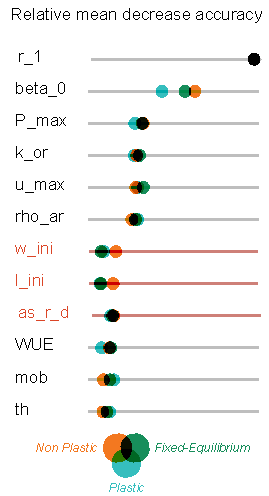
\includegraphics[width = \textwidth]{./2_PP/Figures/importance.pdf}
%\caption{Relative importance of main variables for the three main allocation algorithms (\textcolor{myOrange}{non plastic}, \textcolor{myGreen}{fixed-equilibrium} & \textcolor{myBlue}{plastic}).}
%\end{marginfigure}

PCA performed for \textit{non plastic} algorithm only on parameter values reveals that important parameters are also the dominant variables that shapes the selected subspace. Two main axis seem to correspond to the criterion variables. Species cannot be distinguished on the two main component space, neither on 1 or 2D species specific parameters space (l\_ini, w\_ini, w\_ini vs l\_ini, as\_s\_d, as\_r\_d, as\_r\_d vs as\_s\_d) despite small variations in distribution shapes between species.\\

\paragraph{Variable responses}
% Response of the two main vairables to main parameters.
% Biomass
Total biomass is particularly sensitive to exchange rate parameters, but also tissue respiration cost (\texttt{r\_1)}. There is a notable difference in growth maxima between the two conditions in favour of wet conditions, in line with observed data.  Growth response curves are similar for all allocation algorithm. ?is there a lower difference between conditions for plastic algos? Growth is only weakly related to species specific parameters.\\

\begin{figure}\label{fig:sensitivity_BM}
\includegraphics[width = \textwidth]{./2_PP/Figures/par_effect_none_BM.pdf}
\caption{Main parameters effect on the total plant biomass. \textit{Non plastic}. One dot represents a parameter set. Not all parameter set are represented as the y axis is limited around the smooth function (loess). Coloured points represent selected parameter sets in the two treatments (\textcolor{myOrange}{dry} and \textcolor{myGreen}{wet}).}
\end{figure}

% RSR
Root:Shoot Ratio (or RMF) strongly responds to species specific parameters under \textit{non plastic} allocation because the memory parameters(\texttt{l\_ini} and \texttt{w\_ini}) is the way plant control its RSR ratio. For other allocation rules, species specific parameters have little control over RSR. Surprisingly, the photosynthetic capacity has stronger influence on the ratio than the root maximum exchange rate.


\begin{figure}\label{fig:sensitivity_RSR}
\includegraphics[width = \textwidth]{./2_PP/Figures/par_effect_none_RSR.pdf}
\caption{Main parameters effect on the total plant Root Mass Fraction (RMF). \textit{Non plastic}}
\end{figure}

% TAU
The species specific parameters \texttt{tau} does not emerge as a influencing parameter at the global scale for any of the two flexible allocation rules.

\paragraph{Root shoot ratio and plasticity}

While little to no difference in RSR was expected for \textit{non plastic} allocation rules, both \textit{fixed-equilibrium} and \textit{plastic-optimisation} allocation rules allow for changes in RSR. Nevertheless, no stable change in RSR is observed in any of the simulations. Fluctuations are present but consist in stable oscillations between two fixed values, synchronized with water variations. These rapid adaptations of the relative proportion of roots denote a high flexibility of plant phenotypes in \model.


%\begin{figure}\label{fig:comparison_RSR}
%\includegraphics[width = \textwidth]{./2_PP/Figures/RSR_full_sim.pdf}
%\caption{Comparison of simulated values (over time) of RSR with real species RSR in two contrasting conditons. Because there is no plasticity or ontogeny, the simulated plant do not express any chagnes in RSR}
%\end{figure}

\subsection{Discussion}

\paragraph{Growth and strategy space}

\textbf{Growth is reproduced, but only for one species, not full strategy space.}

\paragraph{}

\textbf{Sensitivity of different variable to the parameters make sense and align with the two criterion of selection (that work with the independence of trade-off).}

\paragraph{More complex plasticity?}

ROle of tau

filtering on RSR to test if plasticity improved selection of parameters, = is an essential part of platn functioning.\\
Change in modelling paradigm. Bayesian paradigm where the information is contained in data and revealed by the structure of the model. Go for simulation experiment approaches where the model is used as a simulation tool and results as new data. The emerging patterns inform us on the impact of the modelled mechanisms (even if they do not totally match the data). Model as an understanding tool.\\
While many ways of simulating the phenotypic plasticity can be proposed, the parsimony is privileged and this representation is enough to understand the impact of related processes shared by any representation of phenotypic plasticity is the developed framework.

\textbf{Root shoot ratio changes were not captured by the model. The structure of the plasticity mechanisms does not work with the given watering cycle. Needs to add one parameter for reactivity.}

% ##################################################################################
\section{Individual level behaviour and properties}


Calibration and sensitivity analysis give information on the main processes of plant growth, but the general effects of the allocation rules on plant growth are not fully identified. In addition, because the parameter filtering processes was limited to individual plants, and the response of species specific parameters dependent on other parameters of the model, the effects of these species specific parameters should further be investigated. The objective of this part is to set better understanding on the role of \textemph{allocation rules} and species \textemph{memory} (for "plastic" allocation algorithm only) on plant development as basis for interpretation of plasticity effects in following chapters.


%Proof of concept
\subsection{Method}


%\paragraph{Strategy diversity filtering}
%To further reduce the number of parameter sets considered, we proceeded in an additional filtering step. Because the first filtering was conduced for only one strategy over the whole 4D strategy space (l\_ini,  w\_ini, as\_s\_d, as\_r\_d) it is necessary to verify that other strategies do not lead to potential Darwinian demon. This should be limited by the choice of priors, while at the same time promoted by the selection of parameters increasing growth to counter balance potential unfitted strategies\footnote{Better do that beforehand than after... But I guess it's too late now.}.

\paragraph{Allocation algorithms}
The effect of allocation on phenotypic development is investigated thanks to pot simulations (see Methods in \ref{section:calibration}) of 100 days in 3 watering treatment: 2mm, 8m and 16mm per day. To avoid drift in the phenotype due to allocation algorithm (see paragraph \ref{subsection:memory} on phenotypic determination), simulations where run a first time, then rerun with default specific traits matching traits at the end of the first simulation set. All four algorithms are simulated.

\paragraph{Memory \& phenotype}
Memory plays a determining role in phenotypic development under "plastic" allocation rules. The effect of this memory alone (environmental cues ignored by setting \texttt{tau} to 1) on the default phenotype is explore for diverse memories (9 values on the two axis from 0.1 to 1 later scaled to the maximum area exchange rates for model parameter set considered, or 81 values) for each accepted parameter set.

\subsection{Results}

think of a "showtime" visualisation that shows how growth and traits are impacted by allocation rules and \texttt{tau}.


\begin{figure}\label{fig:plastic_allocation_trajectory}
\includegraphics[width = \textwidth]{./2_PP/Figures/memory_effect.pdf}
\caption{Trajectories along time in the strategy space of 5 plants with different memories. After 10 days, all plants have converged toward the estimated optimum.}
\end{figure}

\begin{figure}\label{fig:memory_n_phenotype}
\includegraphics[width = \textwidth]{./2_PP/Figures/par_v_2D_points.pdf}
\caption{Impact of species memory on final phenotype in case of fully plastic allocation. Each point corresponds to a plant phenotype for a memory syndrome for a given parameter set. Colours denote the memory syndromes.}
\end{figure}


\begin{figure}\label{fig:w_ini_p_as_r}
\includegraphics[width = \textwidth]{./2_PP/Figures/w_ini_p_as_r.pdf}
\caption{Effect of memory of water availability on proportion of active tissues in root.}
\end{figure}

Strong effect with saturation: optimum. 

\begin{figure}\label{fig:w_ini_p_as_s}
\includegraphics[width = \textwidth]{./2_PP/Figures/w_ini_p_as_s.pdf}
\caption{Effect of memory of water availability on proportion of active tissues in shoot.}
\end{figure}
There is also a positive effect, that is smoother and have lower values. Same pattern for light memory respectively with proportion of active tissues in shoot, and proportion of active tissues in roots.


\subsection{Discussion}
\paragraph{Allocation rules, plasticity and performance}

include figure from "showtime" data to illustrate the differences between allocation algorithms.

\textbf{Allocation rules are extremely important as they reduce the phenotypic space explore. Without even considering plasticity. Need a good understanding of the performance within the phneotypic landscape. Plus there is a need for alignment between starting phenotype and endpoint. Will also affect how plasticity is driven.}

\paragraph{Fast slow strategy and allocation trade-off}

... nothing here, the idea was to show that the "strategy" of the species conduce to slow and fast archetypes.

\textbf{Allocation trade-off allow for strategies from the fast-slow spectrum to arise, independently for shoot and root, in coherent framework. Potential effect of other strategy axis can be analysed alongside this trade-off, even if they affect composite traits like SLA or SRL.}

\paragraph{Memory and phenotypes}

 The symmetry and the curves shapes suggest that resource related organ is more sensitive and that "apparent" increase in resource availability promote more exploitative strategy.\\

For each parameter set the alpha shape of the volume could be drawn to have an idea on how parameters impact potential functional diversity.


\textbf{Memory is a strong enough driver to control plant organ strategy. The effect of overall activity should be studied too and considered if memory is used to determine the default phenotype.)}

% ##################################################################################
\chapter{Individual performance, plasticity and variable conditions}
\section{Individual performance: between strategy, memory and plasticity}

Question I try to answer: (use of schematics ?)

\subsection{Method}

\paragraph{Strategy space sampling}
Idea, having an idea on how the 

\paragraph{Simulation set-up}
Two climatic conditions. ... Watts per square metters and .. mm, days of 15h. Low resource availability conditions correspond to a reduction by a factor 4 of resource influx, but the day length was conserved.

\subsection{Results}


\begin{figure}\label{fig:w_ini_p_as_r}
\includegraphics[width = \textwidth]{./2_PP/Figures/plot_BM_allocation.pdf}
\caption{Effect of plasticity and resource availability on average biomass of living species.}
\end{figure}
Biomass is relative to best performing non plastic plant (to remove the general parameter set effect on growth) and compare (within each condition) the effect of allocation algorithm. Plasticity lead to an increase of average relative biomass, especially full plasticity. However, few values above 1, in fixed conditions there is real additional value of plasticity compare to fixed allocation.\\

Then talk about convergence. To better subspace, but not the optimum.

\subsection{Discussion}

\paragraph{Convergence to subspace}

Somehow I need to talk about the cost of being wrong. Can be observe in the delta heatmap on delta strat and delta w-ini: in this case there is less impact of being wrong of memory if you're good with strategy, because your not in different conditions...\\

Potential effect on diversity: lower functional diversity, increase evenness. Leave highest fitness spot free. Why ? environmental cues or gain function ? Delta between projections ? \\

Anyway, being good is stable conditions may useless if cannot survive or keep gain in other conditions. >> look along gradient if best species keep their rank.\\


\paragraph{Nuances around plasticity}
This analysis was conduced with drastic parameters of plasticity with plastic plants relying only on their perception of external conditions to develop their phenotype. The different results ... different directions and impact on potential diversity.\\
The contrasting responses of the different algorithms highlight the importance of the allocation mechanism. However, the unique framework implemented in \model creates a variety of nuanced responses that are not all explored here. But, the continuous gradient of strategy between species relying on species memory only and species following their perception of external condition should be kept in mind during the interpretation of these results and following.

\paragraph{Resource availability}

results from this part\\
Why we need to go for a gradient.





% ##################################################################################
\section{Plasticity and variability of conditions}
Question I try to answer: (use of schematics ?)

\subsection{Method}

\subsection{Results}

\subsection{Discussion}

\paragraph{Improvement in variable conditions}

\textbf{Phenotypic plasticity }

\paragraph{Heterogeneity of response}

Kichenin (different response to gradient) Doesn't work in this framework: Not so sure about that: depending on your initial memory plants show directional changes toward one phenotype. Yeah, but they should have converged for other conditions too... So, it doesn't work. Might be explained by:
\begin{itemize}
\item different conditions: because heterogeneity and habitat selection, or changes in competition hierarchy;
\item different ways to tackle changes on one dimensions;
\item different weights between mechanisms impacting composite traits, because of the different traits.
\end{itemize}



\paragraph{Extended interpretations}
What about the continuous $\tau$ gradient ?\\
What about interactions and cycles ?



\textbf{The phenotypic plasticity implemented in \model improve the relative performance of multiple strategies by concentrating the plant toward a subspace of higher performance for most of plants. Convergence to a smaller subspace can be assimilated to reduction in phenotypic diversity, but it reduce performance heterogeneity and should favour local plant diversity. .. a few words on dynamics... Meta-community diversity is however reduces by the reduction of potential axis for niche differentiation. Plasticity costs and limits should play major role in the balance between these mechanisms. Community level simulations are needed to further understand the cumulative role of competition, spatial and temporal variability and plasticity costs on phenotypic plasticity influence on plant community dynamics.}

%\section{From individual response to community dynamics}

% Use these notes to extend the discussion and add some outlooks
%
%\section{Niche response}
%
%
%Obj1: understand how resource use mechanisms and allocation algorithms shape the environmental potential niche in the context of the model.\\
%H1: strategy and memory affect niche in two ways if we suppose they are independent: shape and position. Strategy mostly affect shape (width and height) while memory (and so root:shoot ratio) affect mostly position.\\
%H1': there is strong link between strategy and memory in the case of optimisation allocation that increase niche height and might reduce its width.\\
%Obj2: understand the role of plasticity on the niche and if the effect in the same for all strategies/memories.\\
%H2: the plasticity increase niche width but not height (as phenotype is optimum at the center of the niche where memory match the resource availability).
%
%Stability and efficiency trade-off. Niche heigh and width and relationship with the strategy. How does plasticity affect that ? Does it increase the height and widen niches ? What does that mean for coexistence ?\\
%Hopefully higher niche would go with unstable niche.
%%
%%\section{Transitivity and competition}
%%1 vs 1 interactions\\
%%Is the resource competition transitive ? How does niche widening impact that, does plasticty change competition interaction. Is it related to the trait distance ? (don't think so)
